\begin{figure}
%	 pgfplots style "prerocessingexperimentdefault"
		\pgfkeys{/pgfplots/preprocessingexperimentdefault/.style={
				width=\linewidth,
				height=1.4\linewidth,
				every axis plot/.append style={line width = 1.2pt},
				tick pos = left,
				xmajorticks = true,
				ymajorticks = true,
				ylabel near ticks,
				xlabel near ticks,
				xtick align = inside,
				ytick align = inside,
				legend cell align = left,
				legend columns = 1,
				legend pos = south east,
				legend style = {
					fill opacity = 0.9,
					text opacity = 1,
					font = \small,
				},
				xticklabel style = {font = \small, inner xsep = -5ex},
				xlabel style = {font = \small},
				axis line style = {black},
				yticklabel style = {font = \small, inner ysep = -4ex},
				ylabel style = {font = \small},
				title style = {font = \small, inner ysep = -3ex},
				grid = major,
				grid style = {dashed}
			}
		}
	
	\centering
	\begin{subfigure}[t]{0.46\textwidth}
		\begin{minipage}{.49\textwidth}
			\Cshadowbox{\includegraphics[width = .35\textwidth]{fig/06_preprocessing/fig_samples/cifar10raw_3c3d_sample_00.png}}
			\Cshadowbox{\includegraphics[width = .35\textwidth]{fig/06_preprocessing/fig_samples/cifar10raw_3c3d_sample_01.png}}
	
			\Cshadowbox{\includegraphics[width = .35\textwidth]{fig/06_preprocessing/fig_samples/cifar10raw_3c3d_sample_02.png}}
			\Cshadowbox{\includegraphics[width = .35\textwidth]{fig/06_preprocessing/fig_samples/cifar10raw_3c3d_sample_03.png}}
		\end{minipage}
		\begin{minipage}{.49\textwidth}
			\centering
			%			 customize "zmystyle" as you wish
			\pgfkeys{/pgfplots/zmystyle/.style={preprocessingexperimentdefault,
					ylabel={Gradient Element}
			}}
			\vspace{1.4\baselineskip}
			\input{fig/06_preprocessing/fig_histograms/cifar10raw_3c3d.tex}
		\end{minipage}
		\caption{Normalized Data}
		\label{fig:data-pre-processing_norm}
	\end{subfigure}
	\hfill
	\begin{subfigure}[t]{0.46\textwidth}
		\begin{minipage}{.49\textwidth}
			\Cshadowbox{\includegraphics[width = .35\textwidth]{fig/06_preprocessing/fig_samples/cifar10scale255_3c3d_sample_00.png}}
			\Cshadowbox{\includegraphics[width = .35\textwidth]{fig/06_preprocessing/fig_samples/cifar10scale255_3c3d_sample_01.png}}
			
			\Cshadowbox{\includegraphics[width = .35\textwidth]{fig/06_preprocessing/fig_samples/cifar10scale255_3c3d_sample_02.png}}
			\Cshadowbox{\includegraphics[width = .35\textwidth]{fig/06_preprocessing/fig_samples/cifar10scale255_3c3d_sample_03.png}}
		\end{minipage}
		\begin{minipage}{.49\textwidth}
			\centering
%			 customize "zmystyle" as you wish
			\pgfkeys{/pgfplots/zmystyle/.style={preprocessingexperimentdefault,
					ylabel={Gradient Element}
			}}
			\vspace{1.4\baselineskip}
			% This file was created by tikzplotlib v0.9.8.
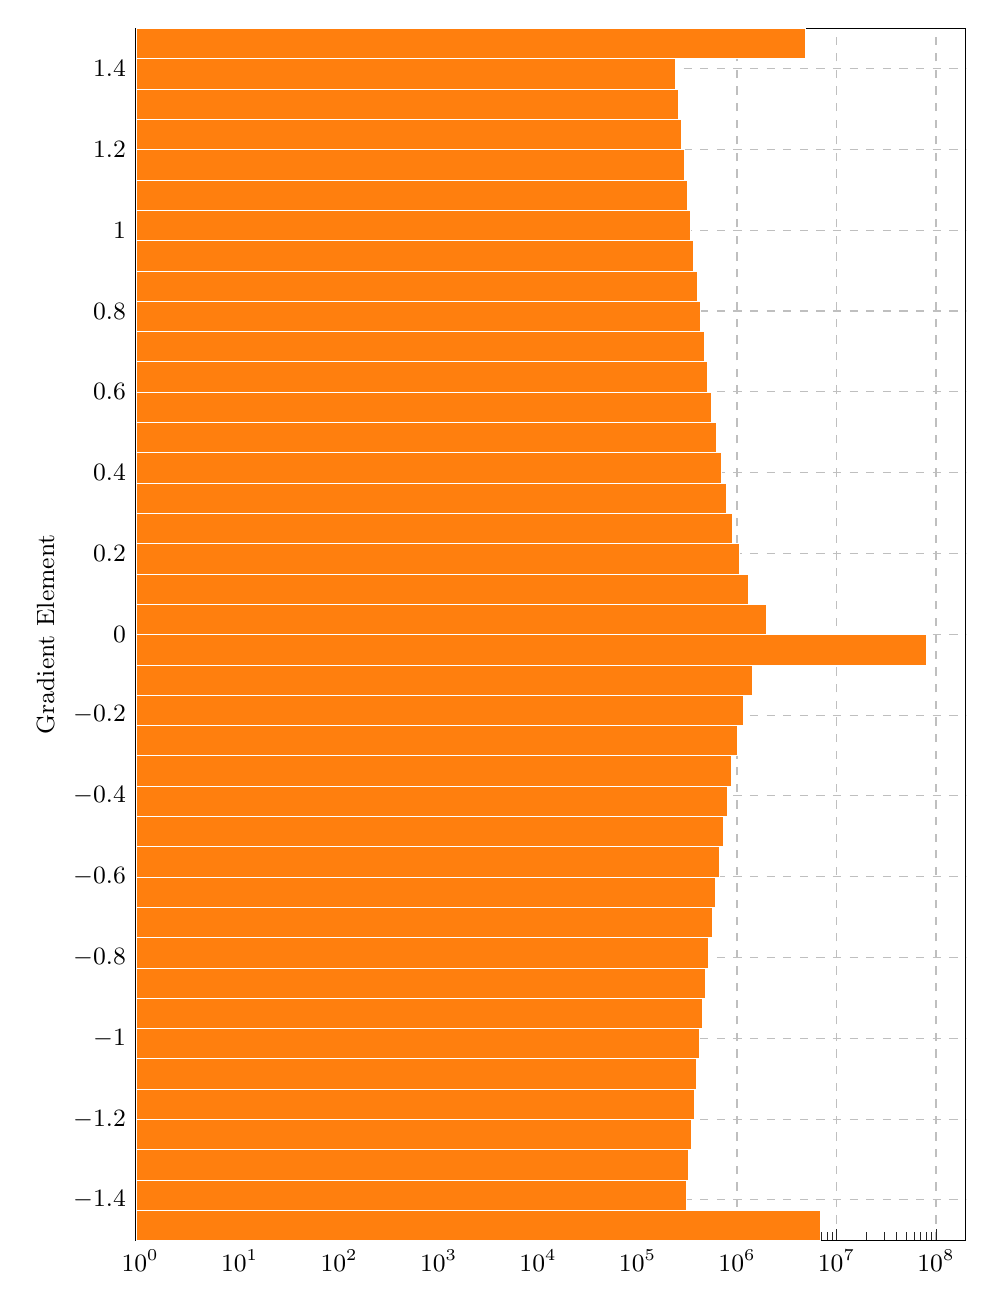
\begin{tikzpicture}

\definecolor{color0}{rgb}{1,0.498039215686275,0.0549019607843137}

\begin{axis}[
axis line style={white},
log basis x={10},
tick align=outside,
xmajorticks=false,
xmin=0.9, xmax=199565229.367149,
xmode=log,
xtick style={color=white!15!black},
ymajorticks=false,
ymin=-1.5, ymax=1.5,
zmystyle
]
\draw[draw=white,fill=color0,line width=0.04pt] (axis cs:0.9,-1.5) rectangle (axis cs:6792656.9,-1.42499995231628);
\draw[draw=white,fill=color0,line width=0.04pt] (axis cs:0.9,-1.42500007152557) rectangle (axis cs:304537.9,-1.35000002384186);
\draw[draw=white,fill=color0,line width=0.04pt] (axis cs:0.9,-1.35000002384186) rectangle (axis cs:322920.9,-1.27499997615814);
\draw[draw=white,fill=color0,line width=0.04pt] (axis cs:0.9,-1.27499997615814) rectangle (axis cs:342177.9,-1.19999992847443);
\draw[draw=white,fill=color0,line width=0.04pt] (axis cs:0.9,-1.20000004768372) rectangle (axis cs:365697.9,-1.125);
\draw[draw=white,fill=color0,line width=0.04pt] (axis cs:0.9,-1.125) rectangle (axis cs:389812.9,-1.04999995231628);
\draw[draw=white,fill=color0,line width=0.04pt] (axis cs:0.9,-1.04999995231628) rectangle (axis cs:417003.9,-0.974999904632568);
\draw[draw=white,fill=color0,line width=0.04pt] (axis cs:0.9,-0.975000023841858) rectangle (axis cs:446173.9,-0.899999976158142);
\draw[draw=white,fill=color0,line width=0.04pt] (axis cs:0.9,-0.899999976158142) rectangle (axis cs:476860.9,-0.824999928474426);
\draw[draw=white,fill=color0,line width=0.04pt] (axis cs:0.9,-0.825000047683716) rectangle (axis cs:514596.9,-0.75);
\draw[draw=white,fill=color0,line width=0.04pt] (axis cs:0.9,-0.75) rectangle (axis cs:555044.9,-0.674999952316284);
\draw[draw=white,fill=color0,line width=0.04pt] (axis cs:0.9,-0.674999952316284) rectangle (axis cs:601849.9,-0.599999904632568);
\draw[draw=white,fill=color0,line width=0.04pt] (axis cs:0.9,-0.600000023841858) rectangle (axis cs:653348.9,-0.524999976158142);
\draw[draw=white,fill=color0,line width=0.04pt] (axis cs:0.9,-0.524999976158142) rectangle (axis cs:715926.9,-0.449999928474426);
\draw[draw=white,fill=color0,line width=0.04pt] (axis cs:0.9,-0.449999988079071) rectangle (axis cs:790634.9,-0.374999940395355);
\draw[draw=white,fill=color0,line width=0.04pt] (axis cs:0.9,-0.374999970197678) rectangle (axis cs:880821.9,-0.299999922513962);
\draw[draw=white,fill=color0,line width=0.04pt] (axis cs:0.9,-0.299999982118607) rectangle (axis cs:996047.9,-0.224999934434891);
\draw[draw=white,fill=color0,line width=0.04pt] (axis cs:0.9,-0.224999964237213) rectangle (axis cs:1158251.9,-0.149999916553497);
\draw[draw=white,fill=color0,line width=0.04pt] (axis cs:0.9,-0.149999968707561) rectangle (axis cs:1410941.9,-0.0749999210238457);
\draw[draw=white,fill=color0,line width=0.04pt] (axis cs:0.9,-0.075000025331974) rectangle (axis cs:79921533.9,2.23517417907715e-08);
\draw[draw=white,fill=color0,line width=0.04pt] (axis cs:0.9,-8.19563865661621e-08) rectangle (axis cs:1965478.9,0.0749999657273293);
\draw[draw=white,fill=color0,line width=0.04pt] (axis cs:0.9,0.0749999210238457) rectangle (axis cs:1289789.9,0.149999968707561);
\draw[draw=white,fill=color0,line width=0.04pt] (axis cs:0.9,0.149999916553497) rectangle (axis cs:1043170.9,0.224999964237213);
\draw[draw=white,fill=color0,line width=0.04pt] (axis cs:0.9,0.224999934434891) rectangle (axis cs:885990.9,0.299999982118607);
\draw[draw=white,fill=color0,line width=0.04pt] (axis cs:0.9,0.299999922513962) rectangle (axis cs:771669.9,0.374999970197678);
\draw[draw=white,fill=color0,line width=0.04pt] (axis cs:0.9,0.374999940395355) rectangle (axis cs:683281.9,0.449999988079071);
\draw[draw=white,fill=color0,line width=0.04pt] (axis cs:0.9,0.449999928474426) rectangle (axis cs:610831.9,0.524999976158142);
\draw[draw=white,fill=color0,line width=0.04pt] (axis cs:0.9,0.524999976158142) rectangle (axis cs:553292.9,0.600000023841858);
\draw[draw=white,fill=color0,line width=0.04pt] (axis cs:0.9,0.599999904632568) rectangle (axis cs:502804.9,0.674999952316284);
\draw[draw=white,fill=color0,line width=0.04pt] (axis cs:0.9,0.674999952316284) rectangle (axis cs:461496.9,0.75);
\draw[draw=white,fill=color0,line width=0.04pt] (axis cs:0.9,0.75) rectangle (axis cs:423747.9,0.825000047683716);
\draw[draw=white,fill=color0,line width=0.04pt] (axis cs:0.9,0.824999928474426) rectangle (axis cs:392145.9,0.899999976158142);
\draw[draw=white,fill=color0,line width=0.04pt] (axis cs:0.9,0.899999976158142) rectangle (axis cs:363396.9,0.975000023841858);
\draw[draw=white,fill=color0,line width=0.04pt] (axis cs:0.9,0.974999904632568) rectangle (axis cs:335621.9,1.04999995231628);
\draw[draw=white,fill=color0,line width=0.04pt] (axis cs:0.9,1.04999995231628) rectangle (axis cs:312992.9,1.125);
\draw[draw=white,fill=color0,line width=0.04pt] (axis cs:0.9,1.125) rectangle (axis cs:291497.9,1.20000004768372);
\draw[draw=white,fill=color0,line width=0.04pt] (axis cs:0.9,1.19999992847443) rectangle (axis cs:273292.9,1.27499997615814);
\draw[draw=white,fill=color0,line width=0.04pt] (axis cs:0.9,1.27499997615814) rectangle (axis cs:255338.9,1.35000002384186);
\draw[draw=white,fill=color0,line width=0.04pt] (axis cs:0.9,1.35000002384186) rectangle (axis cs:240647.9,1.42500007152557);
\draw[draw=white,fill=color0,line width=0.04pt] (axis cs:0.9,1.42499995231628) rectangle (axis cs:4873580.9,1.5);
\end{axis}

\end{tikzpicture}

		\end{minipage}
		\caption{Raw Data}
		\label{fig:data-pre-processing_raw}
	\end{subfigure}
	\caption{\textbf{Same inputs, different gradients; Catching data 
	    bugs with \cockpittitle.} (a) \emph{normalized} ($[0, 1]$) and (b)
    	\emph{raw} $([0, 255])$ images look identical in auto-scaled
	    front-ends like \matplotlib's \texttt{imshow}. The gradient distribution on
	    the \threecthreed model, however, is crucially affected by this
	    scaling.}
	\label{fig:data-pre-processing}
\end{figure}

%%% Local Variables:
%%% mode: latex
%%% TeX-master: "../cockpit_paper"
%%% End:
